\apendice
\chapter{ANÁLISE BIBLIOMÉTRICA}

A bibliometria foi realizada por meio do levantamento bibliográfico relacionado ao tema da pesquisa, utilizando o mecanismo de busca \textit{Google} Acadêmico, e as bases de periódicos \textit{SCOPUS} e \textit{ScienceDirect}. A principal expressão de busca utilizada foi: ``project management''; associada também aos termos: ``project portfolio management'', ``project management office'', ``project management software''; e a tradução destas para a língua portuguesa. A seguir será apresentado os passos desta análise.

\section{Material disponibilizado pelas bases}

O levantamento bibliográfico das fontes impressas e digitais, que não se encontravam disponiveis pela Portal Capes, foi realizado através do portal \textit{ScienceDirect} e do mecanismo Google Acadêmico, que dispõe de bancos de teses e dissertações de instituições específicas, e aprensenta redirecionamento às bases Biblioteca Digital Brasileira de Teses e Dissertações (BDTD), Scientific Electronic Library Online (SciELO).

Ressalta-se ainda que o mecanismo de busca Google Acadêmico também indexa em suas pesquisas as bases de periódicos \textit{SCOPUS} e \textit{ScienceDirect}, permitindo ao usuário avaliar a relevância de citações de um determinado periódico em ambas as bases, e redirecionando o usuário as bases para leitura dos períodicos.

Foi realizada também, uma pesquisa sobre o tema para saber sobre o interesse no mesmo nos ultímos anos, para tanto foi utilizada a ferramenta \textit{Google Trends}. Primeiramente foi utilizada a frase de pesquisa ``project management'' para demonstrar o interesse específico sobre as práticas de GP. O resultado, apresentado no gráfico \ref{trends1}, parte de fevereiro de 2006, se mantendo relativamente contínuo sofrende um leve declínio em janeiro de 2016.


\begin{figure}[!ht]
  \centering
  \scalebox{0.6}{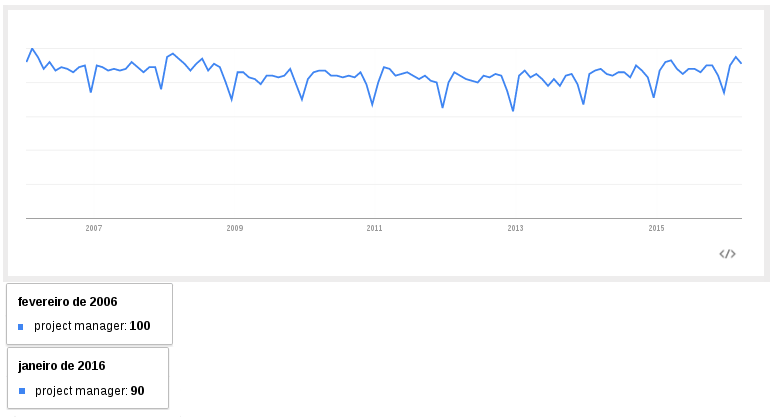
\includegraphics{figuras/trends1}}
  \caption{Interesse sobre práticas de GP ao passar do tempo. Fonte: \textit{Google Trends} (2016).}
  \label{trends1}
\end{figure}


Para saber o interesse geral sobre os demais termos de pesquisa, foram somados os termos: ``project portfolio management'', ``project management office'', ``project management software'', para que assim pudesse haver um comparação sobre o interesse desses com o passar do tempo. O resultado desta pesquisa é apontado no gráfico \ref{trends2}, onde o interesse pela gestão de projetos apresenta um leve declinío, mas contínua representando um bom interesse, enquanto o interesse pelo uso de \textit{software} para GP sobre um declinío considerável e os termos referentes a escritório de gestão de projetos e gestão de portfólio se mantem equilibrados ao longo do tempo.

\begin{figure}[!ht]
  \centering
  \scalebox{0.6}{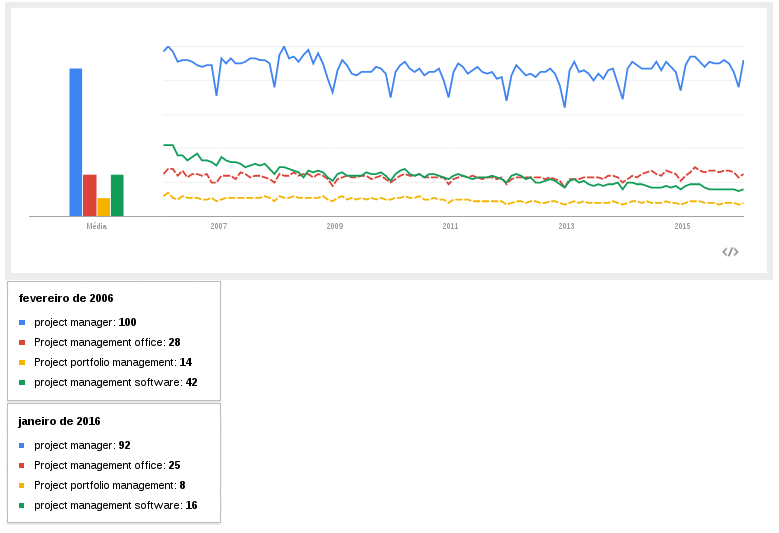
\includegraphics{figuras/trends2}}
  \caption{Interesse sobre demais práticas de GP ao longo do tempo. Fonte: Google \textit{Trends} (2016).}
  \label{trends2}
\end{figure}


Os indicadores bibliométricos escolhidos foram os seguintes: ano de publicação, idiomas, autores e tipos de documento. Seguindo os indicadores escolhidos, a seleção dos artigos foi feita considerando os seguintes critérios:

\begin{itemize}
  \item \textbf{Ano de Publicação:} foi considerado o periodo de 2006 a 2016, isto é, a equivalências aos ultimos dez anos, pois entende-se que este periodo compreende os anos de maior interesse no tema de pesquisa de acordo com mecanismo utilizado.
  \item \textbf{Idiomas:} foi dada preferência ao inglês pela importância que os períodicos desse idioma representaram, entretanto também foram escolhidos períodicos em português pela sua relevância ao tema proposto.
  \item \textbf{Autores:} foram consideradas principalmente publicações de autores mais pesquisados e mais citados.
  \item \textbf{Tipos de Documento:} foi dada preferência a publicações em periódicos, por traduzirem pensamentos mais recentes relativos ao tema de pesquisa.
\end{itemize}


Os trabalhos selecionados a partir da análise bibliometrica, após a aplicação dos indicadores mencionados, encontram-se relacionados no quadro \ref{tabela_autores}.

\begin{longtable}{| p{.20\textwidth} | p{.80\textwidth} |}
  \cline{1-2}
  \cellcolor[HTML]{C0C0C0}{\color[HTML]{000000} Autor(es)} & \cellcolor[HTML]{C0C0C0}{\color[HTML]{000000} Publicação} \\ \hline
    ANDERSEN, B.; HENRIKSEN, B.; AARSETH, W. &
    Benchmarking of project management office establishment: Extracting best practices (2007). \\ \hline
    ATKINSON, R. D.; EZELL, S. J.; STEWART, L. A. &
    The global innovation policy index (2012). \\ \hline
    BROWN, J. T. &
    The handbook of program management: how to facilitate project success with optimal program management (2008). \\ \hline
    BURKE, R. &
    Project management: planning and control techniques (2013). \\ \hline
    CARVALHO, M. M. de; JUNIOR, R. R. &
    Construindo competências para gerenciar projetos: teoria e casos (2008). \\ \hline
    CRAWFORD, J. K. &
    The strategic project office (2010).\\ \hline
    DINSMORE, P. &
    Pmo and best practices (2005). \\ \hline
    DINSMORE, P. C.; CABANIS-BREWIN, J. &
    AMA-Manual de Gerenciamento de Projetos (2009). \\ \hline
    FORTIN, M.-F.; CÔTE, J.; FILION, F. &
    Fundamentos e etapas do processo de investigação (2009). \\ \hline
    GARNICA, L. A.; TORKOMIAN, A. L. V. et al. &
    Gestão de tecnologia em universidades: uma análise do patenteamento e dos fatores de dificuldade e de apoio à transferência de tecnologia no Estado de São Paulo (2009). \\ \hline
    HARTMANN, T.; FISCHER, M.; HAYMAKER, J. &
    Implementing information systems with project teams using ethnographic–action research (2009). \\ \hline
    KENDALL, G. I.; ROLLINS, S. C. &
    Advanced project portfolio management and the PMO: multiplying ROI at warp speed (2003). \\ \hline
    KERZNER, H. R. &
    Project management: a systems approach to planning, scheduling, and controlling (2013). \\ \hline
    LIBERATORE, M. J.; POLLACK-JOHNSON, B.; SMITH, C. A. &
    Project management in construction: Software use and research directions (2001). \\ \hline
    LUNDVALL, B. A. &
    Políticas de inovação na economia do aprendizado (2010). \\ \hline
    LYCETT, M.; RASSAU, A.; DANSON, J. &
    Programme management: A critical review (2006). \\ \hline
    MEREDITH, J. R.; JR, S. J. M. &
    Project management: a managerial approach (2011). \\ \hline
    PEMSEL, S.; WIEWIORA, A. &
    Project management office a knowledge broker in project-based organisations (2013). \\ \hline
    PMI &
    The standard for portfolio management (2006). \\ \hline
    PMI &
    A guide to the project management body of knowledge - pmbok (2014). \\ \hline
    PRADO, D. &
    Mmgp-um modelo brasileiro de maturidade em gerenciamento de projetos (2006). \\ \hline
    RAYMOND, L.; BERGERON, F. &
    Project management information systems: An empirical study of their impact on project managers and project success (2008). \\ \hline
    RIJKE, J. et al. &
    Adaptive programme management through a balanced performance/strategy oriented focus (2014). \\ \hline
    SERBAN, M.; STEFAN, R. M. &
    Project management software (2011). \\ \hline
    TURNER, J. R. &
    The handbook of project-based management 2014. \\ \hline
  \caption{Publicações Selecionadas. Autoria própria (2016).}
  \label{tabela_autores}
\end{longtable}
